\documentclass[t]{beamer}
\usetheme{CMU}

\subtitle{Master Thesis Proposal}
\date{\today}
\author[]{Dalong Cheng\textless dalongc@andrew.cmu.edu\textgreater}
\institute{Institution (Not Used)}

\begin{document}
\maketitle

\begin{frame}
\frametitle{Table of Content}

Table of Content
  \begin{itemize}
    \item Overview
      \begin{itemize}
        \item Why  
        \item What 
      \end{itemize}
    \item Design
      \begin{itemize}
        \item Frontend Design 
        \item Backend  Design
      \end{itemize}
    \item Features
    \item Implementation
    \item Future Works 
  \end{itemize}
\end{frame}

\section{Overview}

\begin{frame}
\frametitle{Background}
\begin{figure}[H] % Example image
\center{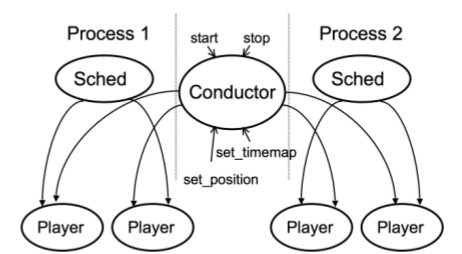
\includegraphics[width=0.4\linewidth]{1.png}}
\caption{Architecture of HCMP}
\label{fig:speciation}
\end{figure}
Human Computer Music Performance(HCMP) Project
  \begin{itemize}
    \item Conductor, Scheduler 
    \item HCMP Player 
  \end{itemize}
\end{frame}

\begin{frame}
\frametitle{Overview}

  \begin{itemize}
    \item Conductor, Schduler 
    \item HCMP Player 
        \begin{itemize}
          \item Especially Tailor For HCMP 
          \item Standalone Mode
          \item Connection Mode 
        \end{itemize}
  \end{itemize}
\end{frame}

\section{Design}

\begin{frame}
\frametitle{Software Architecture}
\begin{figure}[H] % Example image
\center{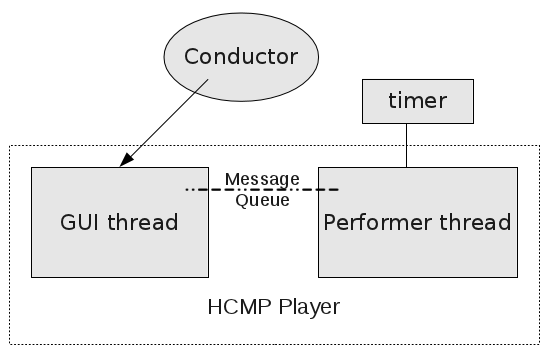
\includegraphics[width=0.6\linewidth]{2.png}}
\caption{Architecture of HCMP}
\label{fig:speciation}
\end{figure}
\end{frame}

\begin{frame}
\frametitle{Control Thread Design}
\begin{figure}[H] % Example image
\center{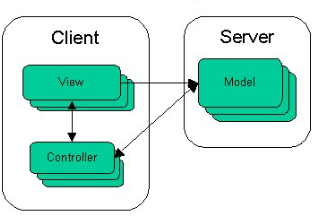
\includegraphics[width=0.4\linewidth]{5.png}}
\caption{Fontend Design}
\label{fig:speciation}
\end{figure}
GUI thread 
  \begin{itemize}
    \item Classic client/server model
    \item Response to user action 
    \item Update canvas based on backend response  
  \end{itemize}

\end{frame}

\begin{frame}
\frametitle{Performer Thread Design}
Performer thread
  \begin{itemize}
    \item Communicate with GUI thread via message queue 
    \item Execute predefine command from GUI thread 
    \item Update canvas based on backend response  
    \item Sample API
  \end{itemize}
  \begin{figure}[H] % Example image
    \center{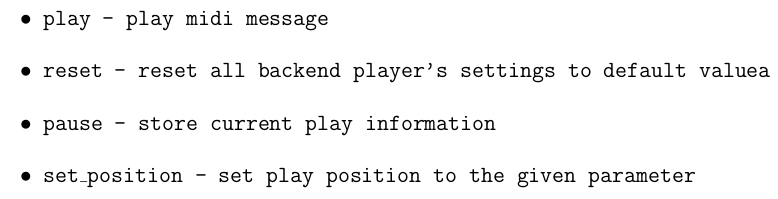
\includegraphics[width=0.8\linewidth]{6.png}}
  \end{figure}
\end{frame}

\section{Features}
\begin{frame}
\frametitle{Network API Support}
  \begin{itemize}
    \item Fully support network control 
    \item GUI thread will be a proxy for backend  
    \item Sample API
  \end{itemize}
   \begin{figure}[H] % Example image
    \center{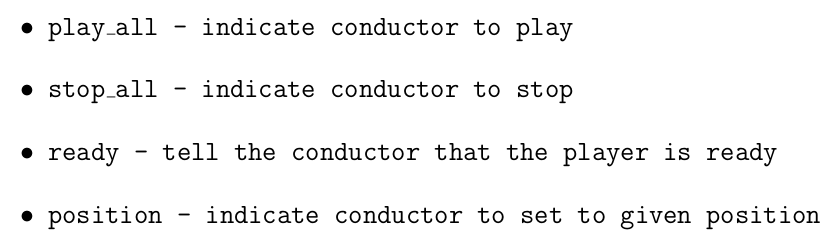
\includegraphics[width=0.8\linewidth]{7.png}}
  \end{figure}
\end{frame}

\begin{frame}
\frametitle{Data Visualization}
\begin{figure}[H] % Example image
\center{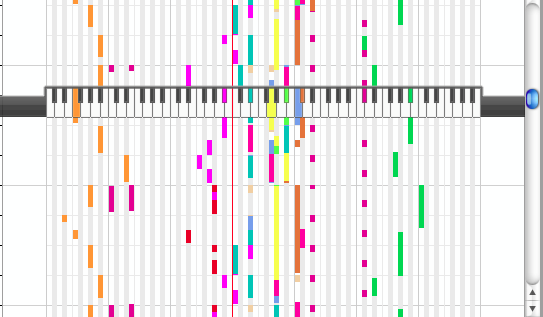
\includegraphics[width=0.5\linewidth]{3.png}}
\caption{Midi data display integrated with virtual keyboard}
\label{fig:speciation}
\end{figure}

\begin{itemize}
  \item Map different track with color 
  \item Map midi to note on keyboard  
  \item a Intuitive visualization effect 
\end{itemize}

\end{frame}

\begin{frame}
\frametitle{A Midi Score Library}
\begin{figure}[H] % Example image
\center{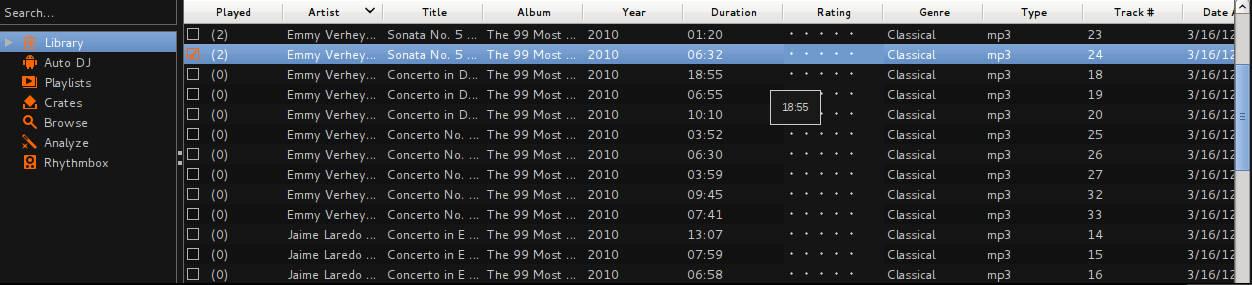
\includegraphics[width=0.6\linewidth]{4.png}}
\caption{HCMP player audio library}
\label{fig:speciation}
\end{figure}

\begin{itemize}
  \item a ''Project'' file to store user setting 
  \item Manage all the user audio  
  \item Support fetch midi from website  
\end{itemize}
\end{frame}

\section{Implementation}
\begin{frame}
\frametitle{Implementation}
\begin{itemize}
  \item wxWidget for GUI part   
  \item Use Serpent for backend  
  \begin{itemize}
    \item Many buildin midi message function 
    \item Support multi-thread 
    \item Fully compatible with HCMP project
  \end{itemize}
\end{itemize}
\end{frame}

\section{Future Works}
\begin{frame}
\frametitle{Future Works}
\begin{itemize}
  \item Fully integrated with score display feature 
  \item Integrate with Dawen Liang's previous work
    \begin{itemize}
      \item music database function into user audio library  
    \end{itemize}
\end{itemize}
\end{frame}

\section{Summary}
\begin{frame}
\frametitle{Summary}
\begin{itemize}
  \item Robustness of code is first priority ! 
    \begin{itemize}
      \item develop unit test for all the functional component  
    \end{itemize}
  \item a Engineering project 
  \item a Live performance for the final defense 
\end{itemize}
\end{frame}

\end{document}
